\documentclass{beamer}
\usetheme{Warsaw}
\usecolortheme{beaver}

\title{X MÇG - X Projesi Kavramsal Tasarım Raporu}
\author[Kirli, Kılınç]{Mesih Veysi Kılınç \and
                       Ahmet Kirli}
\date{2018}

\begin{document}

\section[Giriş]{Giriş Bölümü}
\frame{\titlepage}

\begin{frame}
\frametitle{İçindekiler}
\tableofcontents
%\tableofcontents[currentsection] just for current section
\end{frame}

\subsection[Takım Organizasyonu]{Takım Organizasyonu}
\begin{frame}
\frametitle{Takım Organizasyonu}
    \begin{columns}[c]
        \column{4in}
        Açıklama
    \end{columns}
    \begin{columns}
        \column{4in}
        \framebox{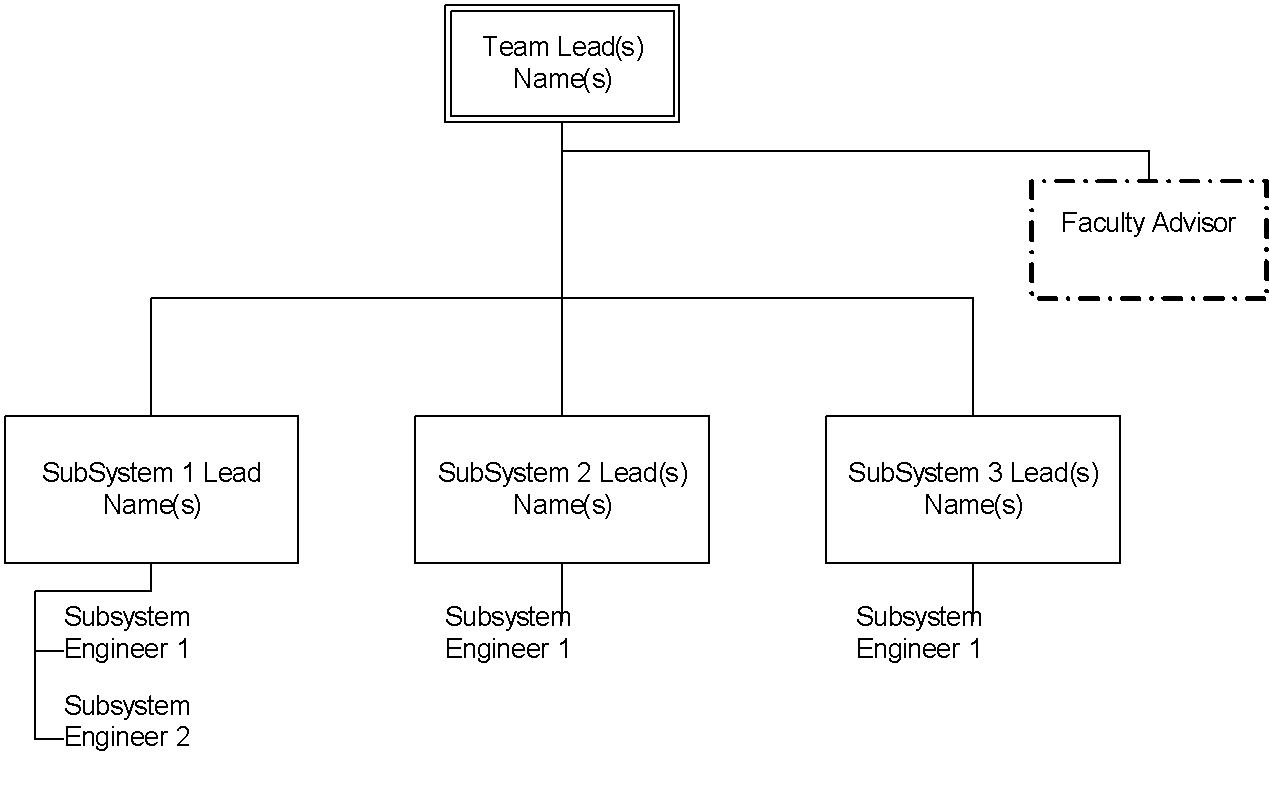
\includegraphics[width=3.75in]{team}}
    \end{columns}
\end{frame}

\subsection{Kısaltmalar}
\begin{frame}
\frametitle{Kısaltmalar}
    \textbf{MÇG}: Mesleki Çalışma Grubu
\end{frame}

\section{Sistem Özeti}
\begin{frame}
\frametitle{Sistem Özeti}
    \begin{columns}[c]
        \column{2in}
        Kısaca sistemin ne işe yaradığından bahsedin
        \column{2in}
        Gerekiyorsa görsel kullanılabilir
    \end{columns}
\end{frame}

\subsection[Görev Özeti]{Görev Özeti}
\begin{frame}
\frametitle{Görev Özeti}
    \begin{columns}[c]
        \column{2in}
        Kısaca görevin ne olduğundan bahsedin
        \column{2in}
        Gerekiyorsa görsel kullanılabilir
    \end{columns}
\end{frame}

\subsection[İster Özeti]{İster Özeti}
\begin{frame}
\frametitle{İster Özeti}
    \begin{columns}[c]
        \column{2in}
        Kısaca isterlerin ne olduğundan bahsedin
        \column{2in}
        Gerekiyorsa görsel kullanılabilir
    \end{columns}
\end{frame}

\section{Ödünleşimler (Tradeoff)}
\begin{frame}[fragile]
    \frametitle{Ödünleşimler (Tradeoff)}
    Sistemde bulunan ödünleşimlerden bahsedin. 
    Örneğin;
    İsterlerde yer alan şu maddeden dolayı kullanmamız gereken motor için ödünleşimler şunlardır:
    \begin{itemize}
        \item
        Motor gücü / motor ağırlığı ödünleşiminden dolayı şu motor seçilmiştir. 
        Bu seçim şu şu sebeplerden dolayı bu ödünleşimi en iyi şekilde dengelemektedir.
    \end{itemize}
\end{frame}

\section{Karvramsal Sistem Tasarımı}
\begin{frame}
\frametitle{Karvramsal Sistem Tasarımı}
Sistem tasarimindan bahsedin. Bir çok sayfadan oluşabilir.
\end{frame}

\subsection[Karşılaşılan Problemler]{Karşılaşılan Problemler}
\begin{frame}
\frametitle{Karşılaşılan Problemler}
Sistem tasarlanırken karşılaşıan problemlerden bahsedin
\end{frame}

\section{Sonuç}
\begin{frame}
\frametitle{Sonuç}
Sonuç olarak belirtmek istediklerinizi ekleyin
\end{frame}

\end{document}

